\documentclass[12pt,twoside]{article}
\usepackage{fancyhdr}
\usepackage{light}
\usepackage{float}
\usepackage{subfigure}
\usepackage{enumitem}
\usepackage{graphicx}
\hidesolutions
\RequirePackage{cases}
\showsolutions
\begin{document}
\newcommand{\inductioncase}[1]{
\textbf{#1}
}
\newcommand{\quizz}[2]{
    \vspace*{-2cm}
  \noindent \coursename \hfill #2 \newline
  \coursestaff \vspace{-1.5ex} \newline
  \mbox{} \hrulefill \mbox{}
%  \vspace{-0.15in}
  \begin{center}
    \ifthenelse{\boolean{showsolutions}}
               {\Large \textbf{Quiz #1 Solutions}}
               {\Large \textbf{Quiz #1}}
  \end{center}
  \vspace{-.1in}
  \thispagestyle{plain}
  \pagestyle{myheadings}
  \thispagestyle{empty}
  \markboth{Quiz #1}{Quiz #1}
  %\coursecopyright
  }
%Solutions are currently incorrect
\quizz{1}{10/25/2016}
\thispagestyle{empty}
\fancyhf{}
\renewcommand{\headrulewidth}{0pt}
\pagestyle{fancy}
\fancyhead[L]{Name: \rule{2in}{0.5pt}}

\begin{itemize}

\item  The quiz is \textbf{closed book}, but you may have one $8.5''  \times 11''$ sheet with notes (either printed or in your own handwriting) on both sides.

\item Calculators and electronic devices (including cell phones) are not allowed.

\item You may assume all of the results presented in class. This does \textbf{not} include results demonstrated in practice quiz material.

\item Write your name on each page of the exam

 \item Please show your work. Partial credit cannot be given for a wrong answer if your work isn't shown.

 \item Write your solutions in the space provided. If you need more space, write on the back of the sheet containing the problem. Please keep your entire answer to a problem on that problem's page.

 \item Be neat and write legibly. You will be graded not only on the correctness of your answers, but also on the clarity with which you express them.

 \item  If you get stuck on a problem, move on to others. The problems are not arranged in order of difficulty.\\


 \textbf{NAME:} \rule{5in}{0.5pt}\\
 
 \textbf{TA:} \rule{5.34in}{0.5pt}\\
 
\centering
\scalebox{1.5}{
\begin{tabular}{|c|c|c|c|}
\hline
\textbf{Problem} & \textbf{Value} & \textbf{Score} & \textbf{Grader} \\\hline
1 & 10 & & \\\hline
2 & 10 & & \\\hline
3 & 10 & & \\\hline
4 & 20 & & \\\hline
5 & 10 & & \\\hline
6 & 10 & & \\\hline
7 & 10 & & \\\hline
8 & 10 & & \\\hline
9 & 10 & & \\\hline
%10 & 10 & & \\\hline
\textbf{Total} & 100 & & \\\hline
\end{tabular}
}
\end{itemize}

\newpage
\begin{problem}{10}
\bparts
\ppart{4}
Use a truth table to prove or disprove $\neg (A \wedge B) \iff (\neg A \vee \neg B)$.
\solution[\vspace{3.5in}]{
\[                                                                                                                                                                                
\begin{array}{c|c|c|c|c|c|c}                                                                                                                                                   
A         & B          &A \wedge B  & \neg (A \wedge B) &\neg A  &\neg B  &\neg A \vee \neg B\\ \hline
\true     &\true       & \true      & \false            & \false & \false & \false \\
\true     &\false      & \false     & \true             & \false & \true  & \true \\                                                                                                         
\false    &\true       & \false     & \true             & \true  & \false & \true \\
\false    &\false      & \false     & \true             & \true  & \true  & \true \\
\end{array}
\]

Comparing the fourth and last colums, we see that the statement is true. \emph{Note:} In fact, this is one of \emph{DeMorgan's Laws}.
}

\item
Translate the following statements from English into propositional logic or vice versa. You may use Prime($p$) to denote that $p$ is prime (i.e., Prime($p$) is True if and only if $p$ is a prime number) in the logical statements.
\begin{enumerate}
\item{[2pts] If $n > 1$, then there is always at least one prime $p$ such that $n < p < 2n$. $n$ is an integer.
\solution[\vspace{2in}]{
The domain is $\mathbb{Z}$.
\begin{equation*}
\forall n. (n > 1) \Rightarrow (\exists p. \text{Prime}(p)  \wedge (n < p) \wedge (p < 2n))
\end{equation*}

\emph{Note:} This is known as \emph{Bertrand's Postulate}
}}
\newpage
\item{[2pts] The domain is $\mathbb{N}$. $\forall m ~ \exists~ p>m. ~\text{Prime}(p) \wedge \text{Prime}(p+2)$
\solution[\vspace{4in}]{
There are infinitely many primes $p$ such that $p+2$ is also prime. \emph{Note:} This is known as the \emph{Twin Prime Conjecture}
}}


\item{[2pts] Let $T$ be the set of TA's, $S$ be the set of students, and $G(x,y) := x \text{ grades } y\text{'s exam}$
\begin{equation*}
\exists ~ t \in T ~ \forall s \in S. ~G(t,s)
\end{equation*}
\solution{
One TA will grade all of the exams. \emph{Note:} This is not a famous law, theorem, or conjecture, but would be quite impressive.
}}
\end{enumerate}
\eparts
\end{problem}


%%%%%%%%%%%%%%%%%%%%%%%%%%%%%%%%%%%%%%%%%%%%%%%%%%%%%

\newpage

%%%%%%%%%%%%%%%%%%%%%%%%%%%%%%%%%%%%%%%%%%%%%%%%%%%%%

\begin{problem}{10}
Prove by induction that $\sum_{k=1}^n k \cdot k!= (n+1)!-1 $ for all integers $n\geq 1$
\solution{

Hypothesis: $P(n) := \sum_{k=1}^n k \cdot k!= (n+1)!-1$

Base case: $n=1$. 
\begin{align*}
\sum_{k=1}^1 k \cdot k! &= (1+1)!-1 \\
1 \cdot 1! &= (2)!-1 \\
1 &= 1
\end{align*}


Inductive step: Assume $P(n)$ holds. We show $P(n+1) := \sum_{k=1}^{n+1} k \cdot k! = (n+2)!-1$
\begin{align*}
& \sum_{k=1}^{n+1} k \cdot k! \\
=& \sum_{k=1}^{n} k \cdot k! + (n+1) \cdot (n+1)!  \\
=& (n+1)!-1 + (n+1) \cdot (n+1)! \\
=& (n+1)!(1 + (n+1)) -1 \\ 
=& (n+1)!(n+2) -1 \\ 
=& (n+2)! - 1 \\ 
\end{align*}

Therefore, by induction, $P(n)$ is true for all $n \geq 1$
}
\end{problem}


%\begin{problem}{10}
%Prove that $(1+x)^k \leq 1+xk$ for every $k \in \mathbb{N}$ for all real $x>-1$
%\solution{
%\begin{align}
%& {} \qquad (1+x)(1+x)^k \ge (1+x)(1+kx)\quad\text{(by hypothesis, since }(1+x)\ge 0) \\
%& \iff (1+x)^{k+1} \ge 1+kx+x+kx^2, \\
%& \iff (1+x)^{k+1} \ge 1+(k+1)x+kx^2. \\
%& \iff (1+x)^{k+1} \ge 1+(k+1)x \\
%\end{align}
%}
%\end{problem}

%%%%%%%%%%%%%%%%%%%%%%%%%%%%%%%%%%%%%%%%%%%%%%%%%%%%%

\newpage

%%%%%%%%%%%%%%%%%%%%%%%%%%%%%%%%%%%%%%%%%%%%%%%%%%%%%


\begin{problem}{10}
Consider the matrix below.
\[
\begin{bmatrix}
    1 & 1 & 1 & 1 \\
    1 & 1 & 1 & 1 \\
    1 & 1 & 1 & 1 \\
    1 & -1 & 1 & 1 \\
\end{bmatrix}
\]

Suppose we are allowed to flip all of the signs of entries in any row or column.  For example, flipping the signs of elements in column two will give the matrix:

\[
\begin{bmatrix}
    1 & -1 & 1 & 1 \\
    1 & -1 & 1 & 1 \\
    1 & -1 & 1 & 1 \\
    1 & 1 & 1 & 1 \\
\end{bmatrix}
\]

Prove that no matter how many operations you perform, there will always be at least one negative entry in the matrix. Do this by identifying an invariant and explain why you can use this invariant to show that at least one -1 will remain in the matrix.  

\solution{
Consider the product of all the elements in this matrix.  We claim that this is invariant under any of the operations provided.  Suppose we flip all the signs of an element in one row.  Then if there were previously $b$ -1's in that row, then there are now $4-b$ -1's in that row and $b$ 1's in that row.  However, $4-b$ and $b$ have the same parity for integer $b = 0, 1, 2, 3, 4$.  Hence, the product remains invariant under a row operation.  A similar argument can be used for the column operation.  Hence as the product is initially -1, the product will always be -1 after any number of row or column operations and so there will always be at least one -1 in the matrix.
}

\end{problem}


%%%%%%%%%%%%%%%%%%%%%%%%%%%%%%%%%%%%%%%%%%%%%%%%%%%%%

\newpage

%%%%%%%%%%%%%%%%%%%%%%%%%%%%%%%%%%%%%%%%%%%%%%%%%%%%%


\begin{problem}{20}
\bparts
\ppart{5} Evaluate $2^{6042}$ mod $63$.

\solution[\vspace{3.5in}]{
We notice that $2 ^ 6 = 64 \equiv 1$ (mod $63$).  Now $6042 = 6 \cdot 1007$.  Hence:

 $2^{6042} = (2^{6})^{1007} \equiv 1$ (mod $63$).
}


\ppart{3} What is $63^{6042}$ mod $6043$? (Hint: 6043 is prime; don't do a messy calculation--it will just waste your time.)

\solution{
By Fermat's little theorem, we can conclude that $63 ^{6042} \equiv 1$ (mod 6043).  
}
%%%
\newpage
%%%
\ppart{6} Give a proof by contradiction that 33 does not have an inverse mod 121.
\solution[\vspace{4in}]{
Suppose that $x$ is the inverse of $33$ mod $121$.  Then we have that $33x - 1 = 121y$ for some integer $y$.  This means that $11 \mid 1$, which is a contradiction.  
}

\ppart{6} Find the inverse of 32 mod 121 in the range $\{ 1, 2, \ldots 120 \}$. (Hint: use the Pulverizer)

\solution{
\[
\begin{array}{ccccrcl}
x & \quad & y & \quad & \rem(x,y) & = & x - q \cdot y \\ \hline
121 && 32 && 25  & = &   121 - 3 \cdot 32 \\
32 && 25 && 7   & = &   32 -  25 \\
&&&&            & = &   32 - (121 - 3 \cdot 32) \\
&&&&            & = &   4 \cdot 32 - 121 \\
25 && 7  && 4   & = &   25 - 3 \cdot 7 \\
&&&&            & = &   (121 - 3 \cdot 32) -
                               3 \cdot (  4 \cdot 32 - 121) \\
&&&&            & = &  4 \cdot 121 - 15 \cdot 32 \\
7 &&  4  && 3   & = &   7 - 4 \\
   &&&&            & = &   (4 \cdot 32 - 121) - (4 \cdot 121 - 15 \cdot 32) \\
&&&&            & = &   19 \cdot 32 - 5 \cdot 121 \\
4 &&  3  && 1   & = &   4 - 3 \\
  &&&&            & = & ( 4 \cdot 121 - 15 \cdot 32 ) - (19 \cdot 32 - 5 \cdot 121) \\
  &&&&            & = &   9 \cdot 121 - 34 \cdot 32 \\
3  && 1  && 0
\end{array}
\]
Hence the inverse of $32$ mod $121$ is just $-34 \equiv 87$ (mod $121$).
}
\eparts
\end{problem}

%%%%%%%%%%%%%%%%%%%%%%%%%%%%%%%%%%%%%%%%%%%%%%%%%%%%%

\newpage

%%%%%%%%%%%%%%%%%%%%%%%%%%%%%%%%%%%%%%%%%%%%%%%%%%%%%


\begin{problem}{10}
A simple graph is said to have width k if you can order the nodes on a straight line so that each node is adjacent to at most k nodes to the left.  Each node can be adjacent to any number of nodes to the right.  

For example, the star graph with 5 nodes shown below has width 1 as can be seen from the ordering shown below the graph.

\begin{figure}[!ht]
\begin{center}
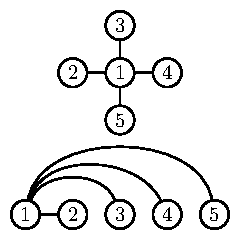
\includegraphics[width=5cm]{StarGraph.pdf}\end{center}
\end{figure}

Prove by induction that any simple graph with width k can be colored in at most k+1 colors.  (Hint: do not induct on k)

\solution{
We induct on the number of vertices $n$.  

\textbf{Base Case:}  Suppose that a we have a graph with $1$ node and width $k$.  Then we only need one color to color our graph and so the graph can be colored in at most $k + 1$ colors.  

\textbf{Inductive Hypothesis:}  Assume that a graph with $n - 1$ nodes and width $k$ can be colored in $k + 1$ colors.  

\textbf{Inductive Step:}  Suppose we have a graph with $n$ nodes and width $k$.  We now show this graph can be colored in at most $k + 1$ colors.  As the graph has width $k$, we can order the nodes from $1, 2, \ldots n$ on a straight line so that each node is adjacent to at most $k$ nodes to the left.  Now if a graph has width $k$, then the graph without one vertex has width $k$. In particular, the subgraph using vertices $1, 2, \ldots n - 1$ has width $k$ and so by our inductive hypothesis, it can be colored using at most $k + 1$ colors.  Now we consider the color of the last vertex $n$.  We know that $n$ is adjacent to at most $k$ nodes in $1, 2, \ldots n-1$.  Hence, we have that we use at most $k$ colors to color the neighbors of node $n$ in the graph, meaning that we have at least one color left over to use for vertex $n$.  Thus, we can color our graph using at most $k + 1$ colors as desired.

As we have proved this for $n$ vertices, by induction, we have that any graph with width $k$ can be colored in $k + 1$ colors.  
}

\end{problem}


%%%%%%%%%%%%%%%%%%%%%%%%%%%%%%%%%%%%%%%%%%%%%%%%%%%%%

\newpage

%%%%%%%%%%%%%%%%%%%%%%%%%%%%%%%%%%%%%%%%%%%%%%%%%%%%%

\begin{problem}{10}
The following questions concern the
following preferences.
\begin{eqnarray*}
girls & \quad & boys \\
\text{Wendy : Stan, Kenny, Butters, Eric} & \quad & \text{Stan: Wendy, Bebe, Heidi, Annie} \\
\text{Bebe : Kenny, Eric, Butters, Stan} & \quad & \text{Kenny : Heidi, Wendy, Bebe, Annie} \\
\text{Heidi : Eric, Butters, Stan, Kenny} & \quad & \text{Butters : Bebe, Wendy, Heidi, Annie} \\
\text{Annie: Butters, Stan, Eric, Kenny} & \quad & \text{Eric : Bebe, Heidi, Wendy, Annie} \\
\end{eqnarray*}
\bparts
\ppart{3}
Is the following a stable marriage? If not, list a rogue couple.
\begin{center}
Wendy -- Stan, Bebe -- Eric, Heidi -- Butters, Annie -- Kenny \\
\end{center}
\solution[\vspace{1.5in}]{
The following is not a stable marriage. Heidi prefers Eric to Butters and Eric prefers Heidi to Bebe.
}

\ppart{7}
Find the matching produced by the stable matching algorithm.

\solution[\vspace{2in}]{
\text{}\\
\textbf{Day 1}\\
Wendy - Stan\\
Bebe - Eric, Butters\\
Heidi - Kenny\\
Annie - no one\\

\textbf{Day 2}\\
Wendy - Stan, Butters\\
Bebe - Eric\\
Heidi - Kenny\\
Annie - no one\\

\textbf{Day 3}\\
Wendy - Stan\\
Bebe - Eric\\
Heidi - Kenny, Butters\\
Annie - no one\\

\textbf{Day 4}\\
Wendy - Stan\\
Bebe - Eric, Kenny\\
Heidi - Butters\\
Annie - no one\\

\textbf{Day 5 - Stable}\\
Wendy - Stan\\
Bebe - Kenny\\
Heidi - Eric\\
Annie - Butters\\
}

\eparts
\end{problem}


%%%%%%%%%%%%%%%%%%%%%%%%%%%%%%%%%%%%%%%%%%%%%%%%%%%%%

\newpage

%%%%%%%%%%%%%%%%%%%%%%%%%%%%%%%%%%%%%%%%%%%%%%%%%%%%%

\begin{problem}{10}
Consider the following graph:

\begin{figure}[!ht]
\begin{center}
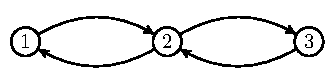
\includegraphics[width=5cm]{PageRankGraph.pdf}\end{center}
\end{figure}

Suppose that each node starts with a PageRank value of $\frac{1}{3}$.  

\bparts
\ppart{3} What weights will the nodes have after one iteration of the Pagerank algorithm?

\solution[\vspace{3in}]{
The values will be $\frac{1}{6}, \frac{2}{3}, \frac{1}{6}$ on vertices 1, 2, 3 respectively.
}

\ppart{7} What will be the PageRank values of each node for the stationary distribution?
\solution{
Suppose $\mu_1, \mu_2, \mu_3$ are the stationary PageRank values on vertices 1, 2, 3 respectively.  Then we must have the following equations:

\begin{equation}
\begin{split}
\mu_1 &= \frac{\mu_2}{2} \\
\mu_2 &= \mu_1 + \mu_3 \\
\mu_3 &= \frac{\mu_2}{2} \\
\mu_1 + \mu_2 + \mu_3 &= 1\\
\end{split}
\end{equation}
Hence by solving the system of equations, we have that $\mu_1 = \mu_3 = \frac{1}{4}$ and $\mu_2 = \frac{1}{2}$. 
}

\eparts

\end{problem}


%%%%%%%%%%%%%%%%%%%%%%%%%%%%%%%%%%%%%%%%%%%%%%%%%%%%%

\newpage

%%%%%%%%%%%%%%%%%%%%%%%%%%%%%%%%%%%%%%%%%%%%%%%%%%%%%


\begin{problem}{10}
Consider the following relation:
$$R = \{(x,y) : x+y=0, x,y \in \mathbb{R}\}.$$
Which of the following properties holds for $R$? If it has the property, prove it. If not, provide a counterexample.

\bparts

\ppart{2} Symmetry.
\solution[\vspace{1.2in}]{
Yes. $x+y=0 \iff y+x=0$
}

\ppart{2} Antisymmetry.
\solution[\vspace{1.2in}]{
No. Counterexample:  $x=-1, y=1$ gives us $xRy$ and $yRx$ but $x \neq y$
}

\ppart{2} Reflexivity.
\solution[\vspace{1.2in}]{
No. Counterexample: For any $x \neq 0$, $\neg xRx$ e.g. if $x=1$,  $x+x \neq 0$ 
}

\ppart{2} Transitivity.
\solution[\vspace{1.2in}]{
No. Counterexample: Let $x = 1, y = -1$ and $z = 1$. Then $x R y$ and $y R z$ but it is not true that $x R z$.
}


\ppart{2} The property of being an equivalence relation.
\solution[\vspace{1.2in}]{
No. It is not reflexive or transitive. 
}

\eparts

\end{problem}


\end{document}

%%%%%%%%%%%%%%%%%%%%%%%%%%%%%%%%%%%%%%%%%%%%%%%%%%%%%

\newpage

%%%%%%%%%%%%%%%%%%%%%%%%%%%%%%%%%%%%%%%%%%%%%%%%%%%%%

\begin{problem}{10}
Prove that a simple graph (i.e. undirected edges) cannot have an odd number of vertices with an odd degree. (Recall that the degree of a vertex is the number of edges incident to that vertex).

\solution{
Sum of all degrees must be even. 
}

\end{problem}

%\begin{problem}{10}
%Suppose we are planning a trip to California for Thanksgiving.  Unfortunately, we are booking our tickets late and so the prices are all really high. Suppose we are given the following list of ticket prices and travel times:
%
%\begin{enumerate}[label=\Alph*]
%\item 600 dollars, 9 hours 20 minutes
%\item 650 dollars, 8 hours 40 minutes
%\item 550 dollars, 9 hours 10 minutes
%\item 575 dollars, 8 hours 20 minutes
%\item 660 dollars, 9 hours 5 minutes
%\end{enumerate}
%
%Our goal is to find the tickets that are the cheapest while minimizing travel time.
%
%\bparts
%\ppart{4} Let's define the following ordering $\leq$. For tickets $i$ and $j$, we say that $i \leq j$ if $i$ is at least as expensive as $j$ is and $i$'s travel time is at least as long as $j$'s travel time. Prove that $\leq$ is a partial order.  
%
%\solution{
%We show that the relation is reflexive:  This is clear, as each ticket is at least as expensive as itself and the travel time per ticket is equal to itself.
%
%We show that the relation is anti-symmetric: Suppose tickets $i,j$ satisfy $i \leq j$ and $j \leq i$. Then ticket $i$ is at least as expensive as ticket $j$ and ticket $j$ is at least as expensive as ticket $j$ so their prices must be equal.  Similarly, ticket $i$'s travel time is at least as long as ticket $j$'s travel time and so ticket $i$ and $j$ have the same travel time.  Hence they are the same ticket.
%
%We show that the relation is transitive: Suppose we have tickets $i, j, k$ such that $i \leq j$ and $j \leq k$.  Then $i$ is at least as expensive as $j$ and $j$ is at least as expensive as $k$, so $i$ is at least as expensive as $k$.  Similarly, $i$'s travel time is at least as long as $j$'s travel time and $j$'s travel time is at least as long as $k$'s travel time.  Hence $i$'s travel time is at least as long as $k$'s travel time.
%}
%
%\ppart{3} Draw the Hasse diagram for the partial order defined above, whose elements are the tickets. You may omit arrows that are self-loops and those that are implied by transitivity.
%
%\solution{
%The Hasse Diagram is below
%
%\begin{figure}[H]
%\begin{center}
%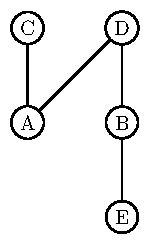
\includegraphics[width=3cm]{PosetGraph.pdf}\end{center}
%\end{figure}
%}
%
%\ppart{3} Find the maximal elements of the poset.  Is there a maximum element? 
%
%\solution{
%Tickets $C$ and $D$ are maximal elements in this poset.  There is no maximum element for this poset.
%}
%\eparts
%\end{problem}

%%%%%%%%%%%%%%%%%%%%%%%%%%%%%%%%%%%%%%%%%%%%%%%%%%%%%

%\newpage

%%%%%%%%%%%%%%%%%%%%%%%%%%%%%%%%%%%%%%%%%%%%%%%%%%%%%



\begin{problem}{10}
The Fibonacci numbers $F_0, F_1, F_2, \dots$ are defined as follows:
\[
F_n \eqdef \begin{cases}
  0               & \mbox{if $n = 0$},\\
  1               & \mbox{if $n = 1$},\\
  F_{n-1} + F_{n-2} & \mbox{if $n >1$}.
\end{cases}
\]

Prove, using strong induction, the following closed-form formula for
$F_n$.
\[
F_n = \frac{p^n-q^n}{\sqrt{5}}
\]
where $p=\frac{1+\sqrt{5}}{2}$ and $q=\frac{1-\sqrt{5}}{2}$.
Hint: note that $p$ and $q$ are the roots of $x^2-x-1=0$, and so
$p^2=p+1$ and $q^2=q+1$.

\solution{
\begin{proof}
We will proceed by strong induction on $n$.  Let the induction
hypothesis, $P(n)$, be that the given closed-form formula holds at
$n$, that is,
\[
F_n = \frac{p^n-q^n}{\sqrt{5}}.
\]

\inductioncase{Base case}($n=0$): $P(0)$ is true, since
\[
\frac{p^n-q^n}{\sqrt{5}}=\frac{p^0-q^0}{\sqrt{5}}=\frac{1-1}{\sqrt{5}}=0=F_0
\]

\inductioncase{Base Case} ($n=1$):  $P(1)$ is true, since
\[
\frac{p^n-q^n}{\sqrt{5}} = \frac{p^1-q^1}{\sqrt{5}} =
\frac{p-q}{\sqrt{5}} = \frac{\sqrt{5}}{\sqrt{5}} = 1 = F_1.
\]

\inductioncase{Inductive Step} ($n > 1$):

Since $0\leq n-1,n < n+1$, we may assume the strong induction
hypothesis that $P(n-1)$ and $P(n)$ are both true.  We will use this
to prove $P(n+1)$.

That is, we may assume
\begin{align}
F_{n-1} & = \frac{p^{n-1}-q^{n-1}}{\sqrt{5}}\label{Fn-1pn-1}\\
F_n & = \frac{p^n-q^n}{\sqrt{5}}\label{Fnpnqn}\\.
\end{align}
From the hint we have that $p^2 = p+1$, which implies that $p^2p^{n-1}
= (p+1)p^{n-1}$ and so
\begin{equation}\label{pn+1pnpn-1}
p^{n+1} = p^n + p^{n-1}.
\end{equation}
Likewise $q^2 = q+1$, and so
\begin{equation}\label{qn+1qnqn-1}
q^{n+1} = q^n + q^{n-1}
\end{equation}
Subtracting~\eqref{qn+1qnqn-1} from~\eqref{pn+1pnpn-1} gives
\[
p^{n+1}-q^{n+1} = p^n-q^n+p^{n-1}-q^{n-1}
\]
and dividing by $\sqrt{5}$ yields
\begin{align}
\frac{p^{n+1}-q^{n+1}}{\sqrt{5}}
 & = \frac{p^n-q^n}{\sqrt{5}}+\frac{p^{n-1}-q^{n-1}}{\sqrt{5}}\notag\\
 & = F_n + F_{n-1} & \text{(by~\eqref{Fn-1pn-1} and~\eqref{Fnpnqn})}\label{pqFF}
\end{align}

But $F_{n+1} = F_n + F_{n-1}$ for $n > 1$ by definition,
so~\eqref{pqFF} implies
\[
F_{n+1} = \frac{p^{n+1}-q^{n+1}}{\sqrt{5}}.
\]
That is, $P(n+1)$ is true in this case as well.

We conclude by strong induction that $P(n)$ holds for all $n \in
\naturals$.
\end{proof}}
%\begin{problem}{10}
%Consider the following matrix $A$:
%
%\[
%A = \begin{bmatrix}
%	1 & 1 \\
%	1 & 0    
%\end{bmatrix}
%\]
%
%Prove by induction that:
%\[
%A^n = \begin{bmatrix}
%	F_{n+1} & F_n \\
%	F_n & F_{n-1}    
%\end{bmatrix}
%\]
%
%where $F_0 = 0$, $F_1 = 1$, and $F_n = F_{n-1} + F_{n-2}$ for all integers $n \geq 2$. $F_i$ for $i  \in \mathbb{N}$ is actually the sequence of Fibonacci numbers, but this knowledge is not needed for the proof.
%
%\solution{
%\textbf{Base Case:}  By the recursion, $F_2 = 1 + 0 = 1$.  Hence as desired:
%
%\[
%A = \begin{bmatrix}
%	F_2 & F_1 \\
%	F_1 & F_0    
%\end{bmatrix}
%\]
%
%\textbf{Inductive Hypothesis:} Assume that for $n = k$, 
%\[
%A^k = \begin{bmatrix}
%	F_{k+1} & F_k \\
%	F_k & F_{k-1}    
%\end{bmatrix}
%\]
%
%\textbf{Inductive Step:} Now for $n = k + 1$:
%
%\[
%A^{k+1} = A \cdot A^{k} = 
%\begin{bmatrix}
% 	1 & 1 \\
%	1 & 0    
%\end{bmatrix} 
%	\begin{bmatrix}
%	F_{k+1} & F_k \\
%	F_k & F_{k-1}    
%\end{bmatrix}  = \\
%\begin{bmatrix}
%	F_{k+1} + F_k & F_k + F_{k-1} \\
%	F_{k+1} & F_{k}    
%\end{bmatrix}  =
%\begin{bmatrix}
%	F_{k+2} & F_{k+1} \\
%	F_{k+1} & F_{k}    
%\end{bmatrix} 
%\]
%
%Hence the statement holds for $n = k+1$, and so it holds for all positive integers $n$ as desired.  
%}
%
%\end{problem}
